\documentclass{ol-softwaremanual}

% Packages used in this example
\usepackage{graphicx}  % for including images
\usepackage{microtype} % for typographical enhancements
\usepackage{minted}    % for code listings
\usepackage{amsmath}   % for equations and mathematics
\setminted{style=friendly,fontsize=\small}
\renewcommand{\listoflistingscaption}{List of Code Listings}
\usepackage{hyperref}  % for hyperlinks
\usepackage[a4paper,top=4.2cm,bottom=4.2cm,left=3.5cm,right=3.5cm]{geometry} % for setting page size and margins
\usepackage{svg} % práce se SVG
\usepackage{xcolor}
\usepackage{dirtree}
\usepackage{pdfpages}


\newif\ifnotes
\notestrue   % ukázat poznámky
%\notesfalse

% příkaz pro poznámky
\newcommand{\note}[1]{%
  \ifnotes
    \textcolor{red}{#1}%
  \fi
}

% Custom macros used in this example document
\newcommand{\doclink}[2]{\href{#1}{#2}\footnote{\url{#1}}}
\newcommand{\cs}[1]{\texttt{\textbackslash #1}}

% Frontmatter data; appears on title page
\title{Treadmill sideshift \\ documentation}
\version{1.0.0}
\author{Martin Kriz}
\softwarelogo{
\includegraphics[width=12cm]{logo.png}}

\begin{document}

\maketitle

\tableofcontents
\listoflistings
\newpage

\section{Introduction}

A PCB developed for a treadmill in the lab to provide lateral movement for testing the camera box. Two identical PCBs are used, controlling both ends of the treadmill.

\newpage
\section{Hardware}

\subsection{Block diagram}
\begin{figure}[h!]
    \centering
    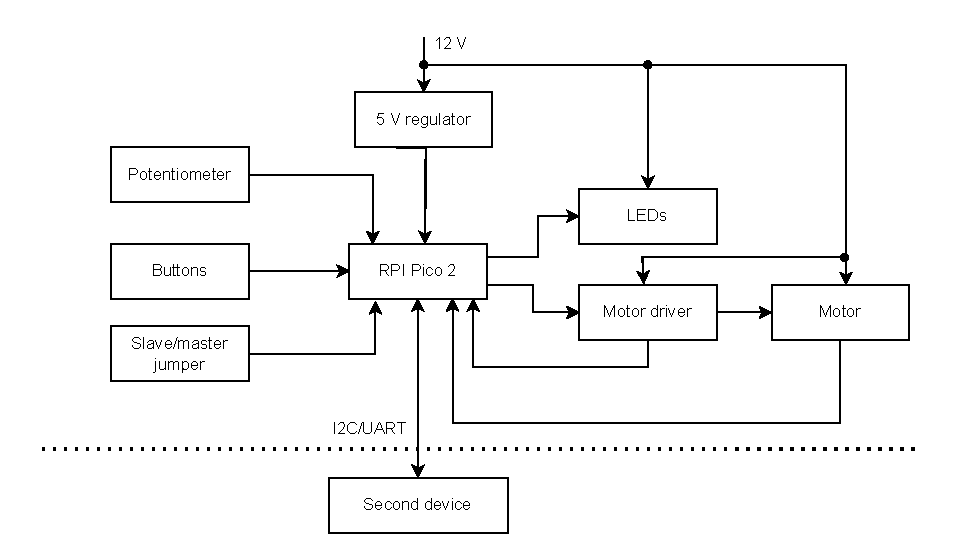
\includegraphics[width=\textwidth]{images/Sideshift-block-diagram.pdf}
    \caption{Block diagram of the treadmill sideshift module.}
    \label{fig:sideshift-block-diagram}
\end{figure}

\subsection{Motor Linak LA14}
Exact model number is Linak 14020130000A0C06:
\begin{itemize}
    \item \textbf{Feedback:} Hall potentiometer
    \item \textbf{Motor type:} 12 V BDC Fast
    \item \textbf{Endstop:} Power switch 
\end{itemize}
The figure \ref{fig:motor_connect} shows the correct connection of the motor to the PCB.
\begin{figure}[h!]
    \centering
    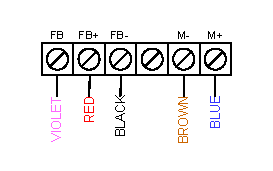
\includegraphics[width=0.5\textwidth]{images/motor_wiring.drawio.pdf}
    \caption{Connecting motor to the PCB.}
    \label{fig:motor_connect}
\end{figure}

\newpage
\subsection{Motor driver DRV8873}
Configuration of the DRV8873 used in this project:

\begin{itemize}
    \item \textbf{Interface:} Hardware
    \item \textbf{Current sensing:} Active over 360 Ohm resistor
    \item \textbf{Control mode:} PH/EN
    \item \textbf{PWM:} Software use 25~kHz
    \item \textbf{Slew rate:} \(13 V/ \mu s \)
    \item \textbf{Current ITRIP regulation:} Enabled
    \item \textbf{Open load diagnostic:} Enabled
\end{itemize}


\begin{figure}[h!]
    \centering
    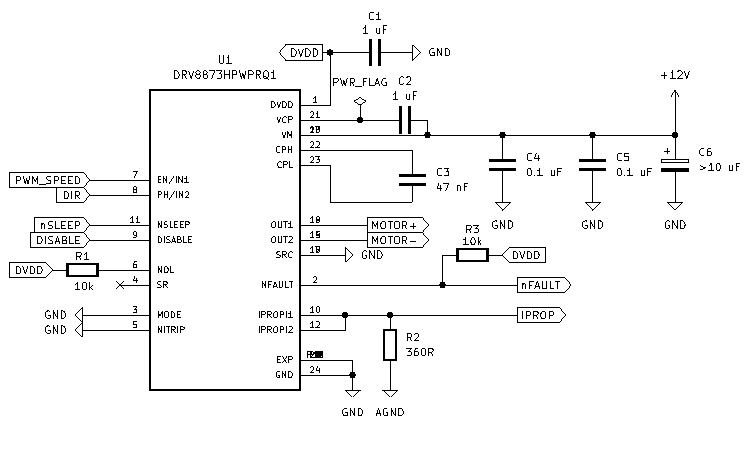
\includegraphics[width=\textwidth]{images/DRV8873H_wiring.pdf}
    \caption{DRV8873H schematic.}
    \label{fig:DRV8873H_wiring}
\end{figure}

\newpage
\subsection{RPi Pico 2}

\begin{figure}[h!]
    \centering
    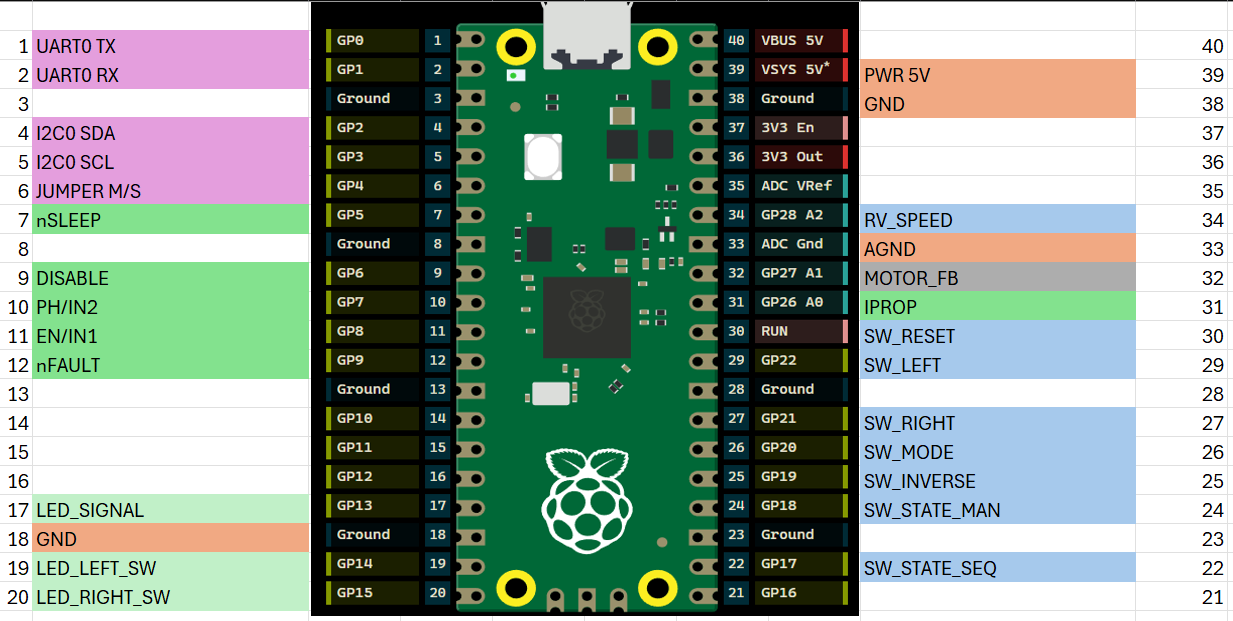
\includegraphics[width=0.9\textwidth]{images/pico_pin_mapping.png}
    \caption{RPi Pico pin mapping.}
    \label{fig:pico_pin_mapping}
\end{figure}

The Raspberry Pi Pico is powered from a 5V regulator and connected through a Schottky diode so that when a USB cable is connected to the Pico, it cannot supply power to the rest of the PCB.

A reset button is placed on the PCB, and when pressed, it grounds the RUN pin, causing the Pico to reset.

\begin{figure}[h!]
    \centering
    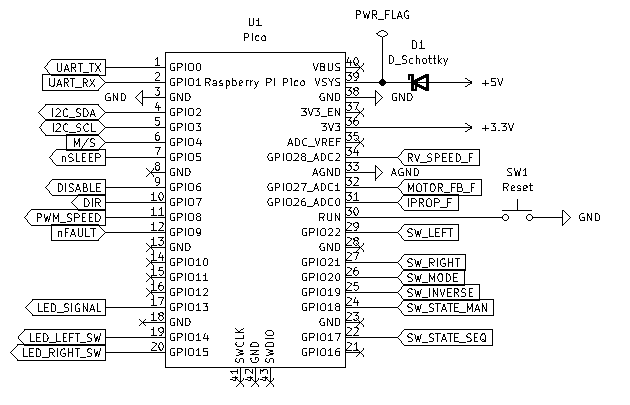
\includegraphics[width=\textwidth]{images/pico_wiring.pdf}
    \caption{RPi Pico schematic}
    \label{fig:pico_wiring}
\end{figure}




\newpage
\subsection{Power supply}
An external 12 VDC power supply is connected to the board, which should be able to provide a current of at least 1.5 to 2 A.


The power input is 12~V is protected by a 5~A fuse based on Table~\ref{tab:power_consumption}, providing protection against reverse polarity and short circuits. In case of reverse polarity, the fuse must be replaced as it will be permanently damaged. As a 5V regulator, the LM7805 is used, and an LED is connected to it to indicate the voltage at the regulator's output. See the schematic in figure \ref{fig:power_schematic}.



\begin{table}[h!]
\centering
\begin{tabular}{|l|c|c|l|}
\hline
\textbf{Component} & \textbf{Supply Voltage (V)} & \textbf{Max Current (mA)} & \textbf{Power Source}\\
\hline
RPI Pico           & 5  & 100  & Regulator (7805) \\
\hline
Driver DRV8833     & 12 & 10   & Power supply \\
\hline
DC motor           & 12 & 2500 & Driver \\
\hline
Motor feedback     & 12 & 1    & Power supply \\
\hline
State LED          & 12 & 20   & Power supply      \\
\hline
Mode button LED    & 12 & 20   & Power supply  \\
\hline
PWR switch LED     & 12 & 20   & Power supply       \\
\hline
\end{tabular}
\caption{Power consumption of individual components}
\label{tab:power_consumption}
\end{table}

\begin{figure}[h!]
    \centering
    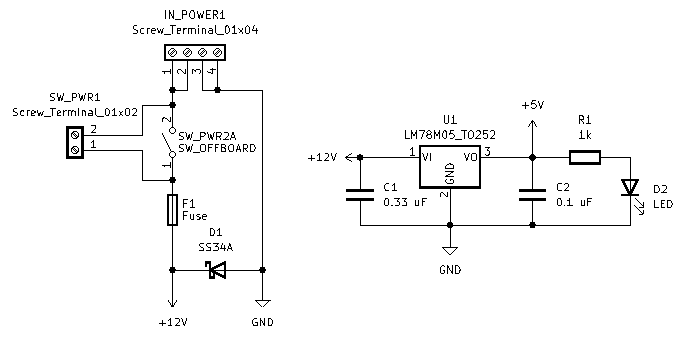
\includegraphics[width=\textwidth]{images/power_schematic.pdf}
    \caption{Power supply schematic.}
    \label{fig:power_schematic}
\end{figure}

\newpage
\subsection{Analog circuits}
All analog signals use simple RC low-pass filters, and their cutoff frequencies are listed in table \ref{tab:rc_filters}. All analog sections also have a separate ground, AGND.

\begin{table}[h!]
\centering
\begin{tabular}{|c|c|c|c|}
\hline
\textbf{Signal} & \textbf{R} & \textbf{C} & \textbf{Cutoff frequency} \\ \hline
Motor feedback & 10 k$\Omega$ & 1 $\mu$F & 15.9 Hz \\ \hline
Potentiometer & 10 k$\Omega$ & 1 $\mu$F & 15.9 Hz\\ \hline
Motor current & 10 k$\Omega$ & 3.3 nF & 4823 Hz\\ \hline
\end{tabular}
\caption{RC Low-pass filters for analog signals}
\label{tab:rc_filters}
\end{table}

\subsubsection{Motor current IPROP}
The motor current is measured using the IPROPI1 and IPROPI2 pins, which are connected together for the purpose of this application. For converting the current into a voltage, the resistor $R_{\text{sense}}$ is used, and its value is determined from the following equation:

 \begin{equation}
	\label{r_sense}
    R_{sense}= \frac{k\cdot U_{max}}{I_0}=\frac{1100 \cdot 3.3}{10} \doteq 360 \; \Omega
\end{equation}

\subsubsection{Motor feedback}
The motor feedback from the LINAK LA14 ranges from 0 to 10\,V; a voltage divider is used to scale it down to 0–3.3\,V for the Raspberry Pi Pico's ADC. In addition, a safety margin is provided so that in the event of a fault, where a voltage of up to 12\,V may appear on the pin, the ADC will not be damaged.
\begin{table}[h!]
\centering
\begin{tabular}{|c|c|c|c|}
\hline
{$U_{in} [V]$} & {$R_1$ [$\Omega$]} & {$R_2$ [$\Omega$]} & {$U_{out} [V]$} \\ \hline
12 & 100k & 36k & 3.18 \\ \hline
\end{tabular}
\caption{Voltage divider for motor feedback input.}
\label{tab:voltage_divider}
\end{table}

\subsection{LEDs}
For panel mounting, the LEDs need to be powered from 12\,V. Therefore, the ULN2004A integrated circuit was used. To set the LED current to approximately 20\,mA, a series resistor of 470\,$\Omega$ was chosen.The LED lights up when a logic high (1) is applied to the corresponding Raspberry Pi Pico pin.

\begin{figure}[h!]
    \centering
    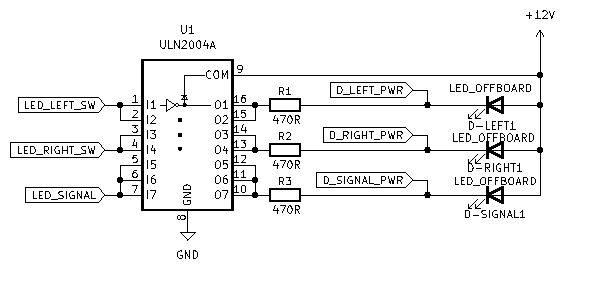
\includegraphics[width=\textwidth]{images/leds_wiring.pdf}
    \caption{LEDs schematic.}
    \label{fig:leds_schematic}
\end{figure}

\newpage
\subsection{Communication}
Communication with the second board is carried out via I\textsuperscript{2}C or UART. When using the I\textsuperscript{2}C bus, it is necessary to set whether the device acts as a master or a slave by means of a hardware jumper. It is necessary to ensure that one board has the jumper set to the slave position and the other board has the jumper set to the master bus position.


\begin{figure}[h!]
    \centering
    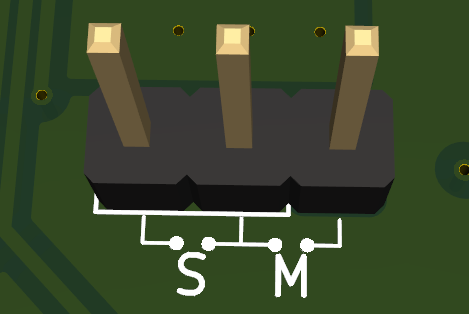
\includegraphics[width=0.2\textwidth]{images/ms_select.png}
    \caption{Master/Slave jumper.}
    \label{fig:ms_select}
\end{figure}

\note{For PCB version v1.0.0, the pin selected for I\textsuperscript{2}C is incorrect, and it is not possible to operate it on the prepared pins. As a temporary solution, the I\textsuperscript{2}C protocol can be used on the UART pins, where Tx corresponds to SDA and Rx corresponds to SCL. Therefore, when switching protocols, it is always necessary to swap the wires.}

\note{
\begin{figure}[h!]
    \centering
    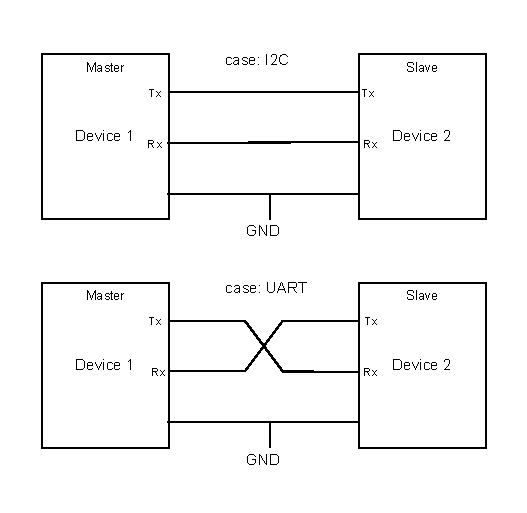
\includegraphics[width=0.63\textwidth]{images/sideshift_master_slave.pdf}
    \caption{\note{Temporary communication wiring.}}
    \label{fig:temp_comm_schematic}
\end{figure}
}




\newpage
\section{Control panel}
\subsection{Front view}
\begin{figure}[h!]
    \centering
    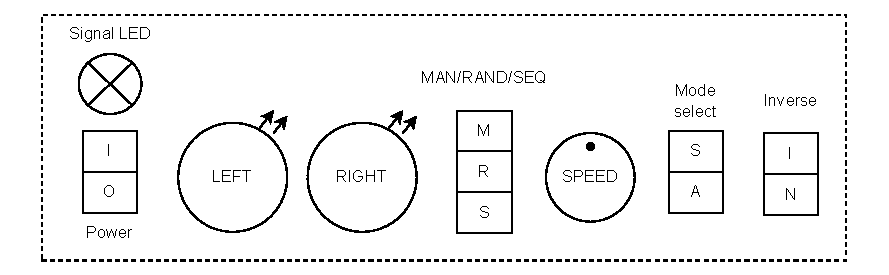
\includegraphics[width=\textwidth]{images/siteshift_frontview.drawio.pdf}
    \caption{Control panel front view.}
    \label{fig:control_panel}
\end{figure}

\subsection{Components}
\begin{description}
    \item[Signal LED] 12 V, 20 mA
    \item[Power switch] A rocker switch rated for at least 2 A
    \item[L/R button] A non-latching push button with 12 V LED backlight.
    \item[State switch] A three-position switch
    \item[Speed potentiometer] 10 k$\Omega$ potentiometer
    \item[Mode/Inverse switch] A two-position switch
\end{description}

\subsection{Wiring}
Each screw terminal for connection is marked with the number 1 on one side; numbering proceeds from that side. An example is shown in figure~\ref{fig:control_panel_wiring}.
\begin{figure}[h!]
    \centering
    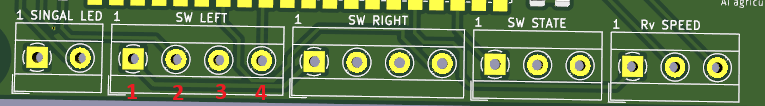
\includegraphics[width=\textwidth]{images/control_panel_wiring.png}
    \caption{Screw terminal numbering.}
    \label{fig:control_panel_wiring}
\end{figure}
\begin{figure}[h!]
    \centering
    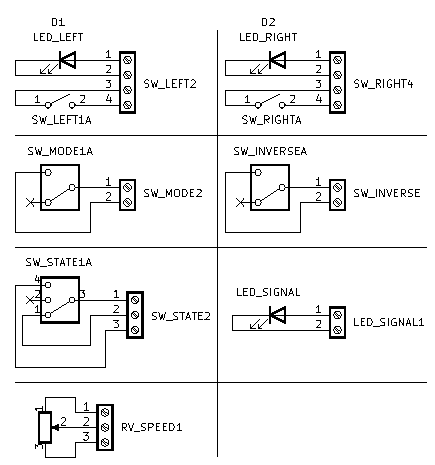
\includegraphics[width=0.8\textwidth]{images/control_panel_schematic.pdf}
    \caption{Control panel connection diagram. Note: This is a connection-only schematic.}
    \label{fig:control_panel_schematic}
\end{figure}

\subsection{Usage}
After turning on the power using the \textbf{power button}, calibration starts automatically. 
Until the calibration is complete, the device cannot be controlled.

The higher a button is placed in this list, the higher its priority.
\begin{description}
    \item[Mode switch] Switches between the state of following the second device synchronous operation (SYN)  
    or the asynchronous state (ASYN), where it is possible to control the device using the    control panel.
    \item[State switch] Three-position switch, allowing switching between manual control, random, and sequential modes.  
    This switch is considered only when ASYN is selected on the previous button.
    \item[L/R buttons] Buttons used to manually move the piston while held.  
    These buttons are active only when the previous switch is set to the manual position.  
    When the buttons are active, the LED backlight is illuminated.
    \item[Speed potentiometer] In asynchronous mode, the potentiometer can be used to set the maximum speed of the piston movement.
\end{description}
The signal LED is active when the device is in any mode other than manual, indicating that the device is active.  
If the device is in synchronous mode and the LED is blinking, this indicates a communication error.


\newpage
\section{Software}

The code is written in the Arduino IDE for the Raspberry Pi Pico2.  
The project structure is as follows:

\dirtree{%
.1 treadmill\_sideshift.ino \DTcomment{Main project file}.
.1 src/.
.1 include/ \DTcomment{Classes used by main hardware handling, algorithms}.
.2 I2CCommunication.h \DTcomment{Provide I2C communication}.
.2 ICommunication.h \DTcomment{Defines communication interface}.
.2 Motor.h \DTcomment{Provide communication with the motor driver}.
.2 MotorFeedback.h \DTcomment{Reading analog feedback from motor}.
.2 OtherDevice.h \DTcomment{Defines communication message, store the last message}.
.2 Pid.h \DTcomment{PID controller with integral windup protection}.
.2 PositionCalculator.h \DTcomment{converts raw ADC readings from a motor piston sensor into a physical position}.
.2 UARTCommunication.h \DTcomment{Provide I2C communication}.
.2 UserInterface.h \DTcomment{handles buttons, potentiometer, and LED indicators}.
.1 test/ \DTcomment{Codes for solo hardware testing, other device simulation}.
.2 ICommunication\_test/.
.2 Motor\_test/.
.2 MotorFeedback\_test/.
.2 SynMode\_test/.
.2 UserInterface\_test/.
}
The properties of the classes are defined in the headers of the individual files.

\subsection{State machine}
\begin{figure}[h!]
    \centering
    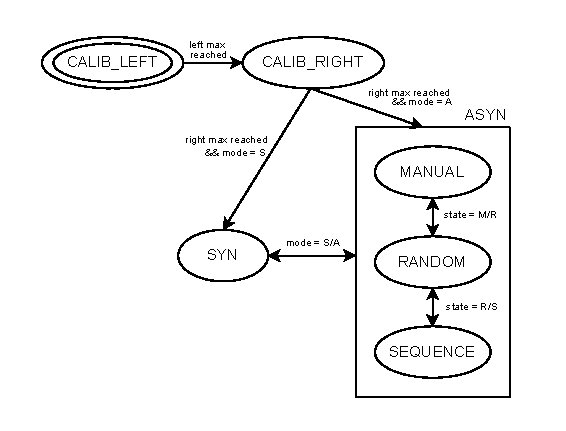
\includegraphics[width=\textwidth]{images/sideshift_state-machine.drawio.pdf}
    \caption{Sideshift state machine.}
    \label{fig:state_machine}
\end{figure}

State description:
\begin{itemize}
    \item \textbf{CALIB\_LEFT} – Initial state, used to find the maximum ADC value of the transducer, which is then stored to determine the exact position of the piston at its extreme end. The maximum is determined by running the motor until its position no longer changes for a certain period of time.
    \item \textbf{CALIB\_RIGHT} – The same, but in this case it concerns the minimum ADC value of the transducer.
    \item \textbf{SYN} – State in which the piston follows the second piston (position is known via communication). A PI controller is used to maintain zero control deviation.
    \item \textbf{MANUAL} – Manual control is active, allowing the piston to be positioned using the L/R buttons. The maximum speed is selected via a potentiometer.
    \item \textbf{RANDOM} – In random mode, a position is selected within the range of the piston rod, and a PI controller drives the rod to the selected position. After reaching the position, the next position is selected randomly. Maximum speed is set via a potentiometer.
    \item \textbf{SEQUENCE} – The piston rod moves left and right, with the maximum speed set via a potentiometer.
\end{itemize}

Transitions between states
\begin{itemize}
    \item \textbf{MAX REACHED} – The maximum (minimum) is considered reached if the motor is driven in one direction, 
    and the ADC converter value does not change by more than the interval defined in the 
    constant \texttt{changeTolerance} during the time interval defined in the constant 
    \texttt{stableThreshold}.
    \item \textbf{STATE and MODE} – These transitions depend on the position of the switches on the control panel.
\end{itemize}

\subsection{Communication}
\subsubsection{Choosing protocol}
For communication, it is necessary to correctly select the protocol, which is chosen in the \texttt{setup} loop.  
One of the following lines must be uncommented:
\begin{verbatim}
comm = new UARTCommunication();
//comm = new I2CCommunication(isMaster);
\end{verbatim}

By enabling the UART protocol, a class is created that handles the communication.  
The protocols must be the same on both boards.

\subsubsection{Message type}
Messages are sent as strings. The \texttt{OtherDevice} class handles this conversion,  
and follows these rules:

\begin{itemize}
    \item The message always starts with the character \texttt{<}.
    \item Values are separated by commas.
    \item The first value is the piston position (\texttt{pos}), represented as a floating-point number with two decimal places.
    \item The second value is the potentiometer reading (\texttt{pot}), represented as an integer.
    \item The third value is the direction (\texttt{dir}), represented as an integer.
    \item The message always ends with the character \texttt{;}.
\end{itemize}

\noindent
An example of a generated message:
\begin{verbatim}
<12.45,75,1;
\end{verbatim}

\noindent
Meaning of the message:
\begin{itemize}
    \item \texttt{pos = 12.45} $\rightarrow$ piston position in millimeters.
    \item \texttt{pot = 75} $\rightarrow$ potentiometer value in percent (75\,\% of maximum speed).
    \item \texttt{dir = 1} $\rightarrow$ piston movement direction.
\end{itemize}

\subsubsection{Communication period}
The communication period can be set by the constant \textit{COMM\_MS} in the main file. By default, it is set and tested to 50 ms.



\newpage
\section{Appendix}

\appendix
\section{Schematic diagram}
\section{PCB layout TOP (red) and BOTTOM (blue)}

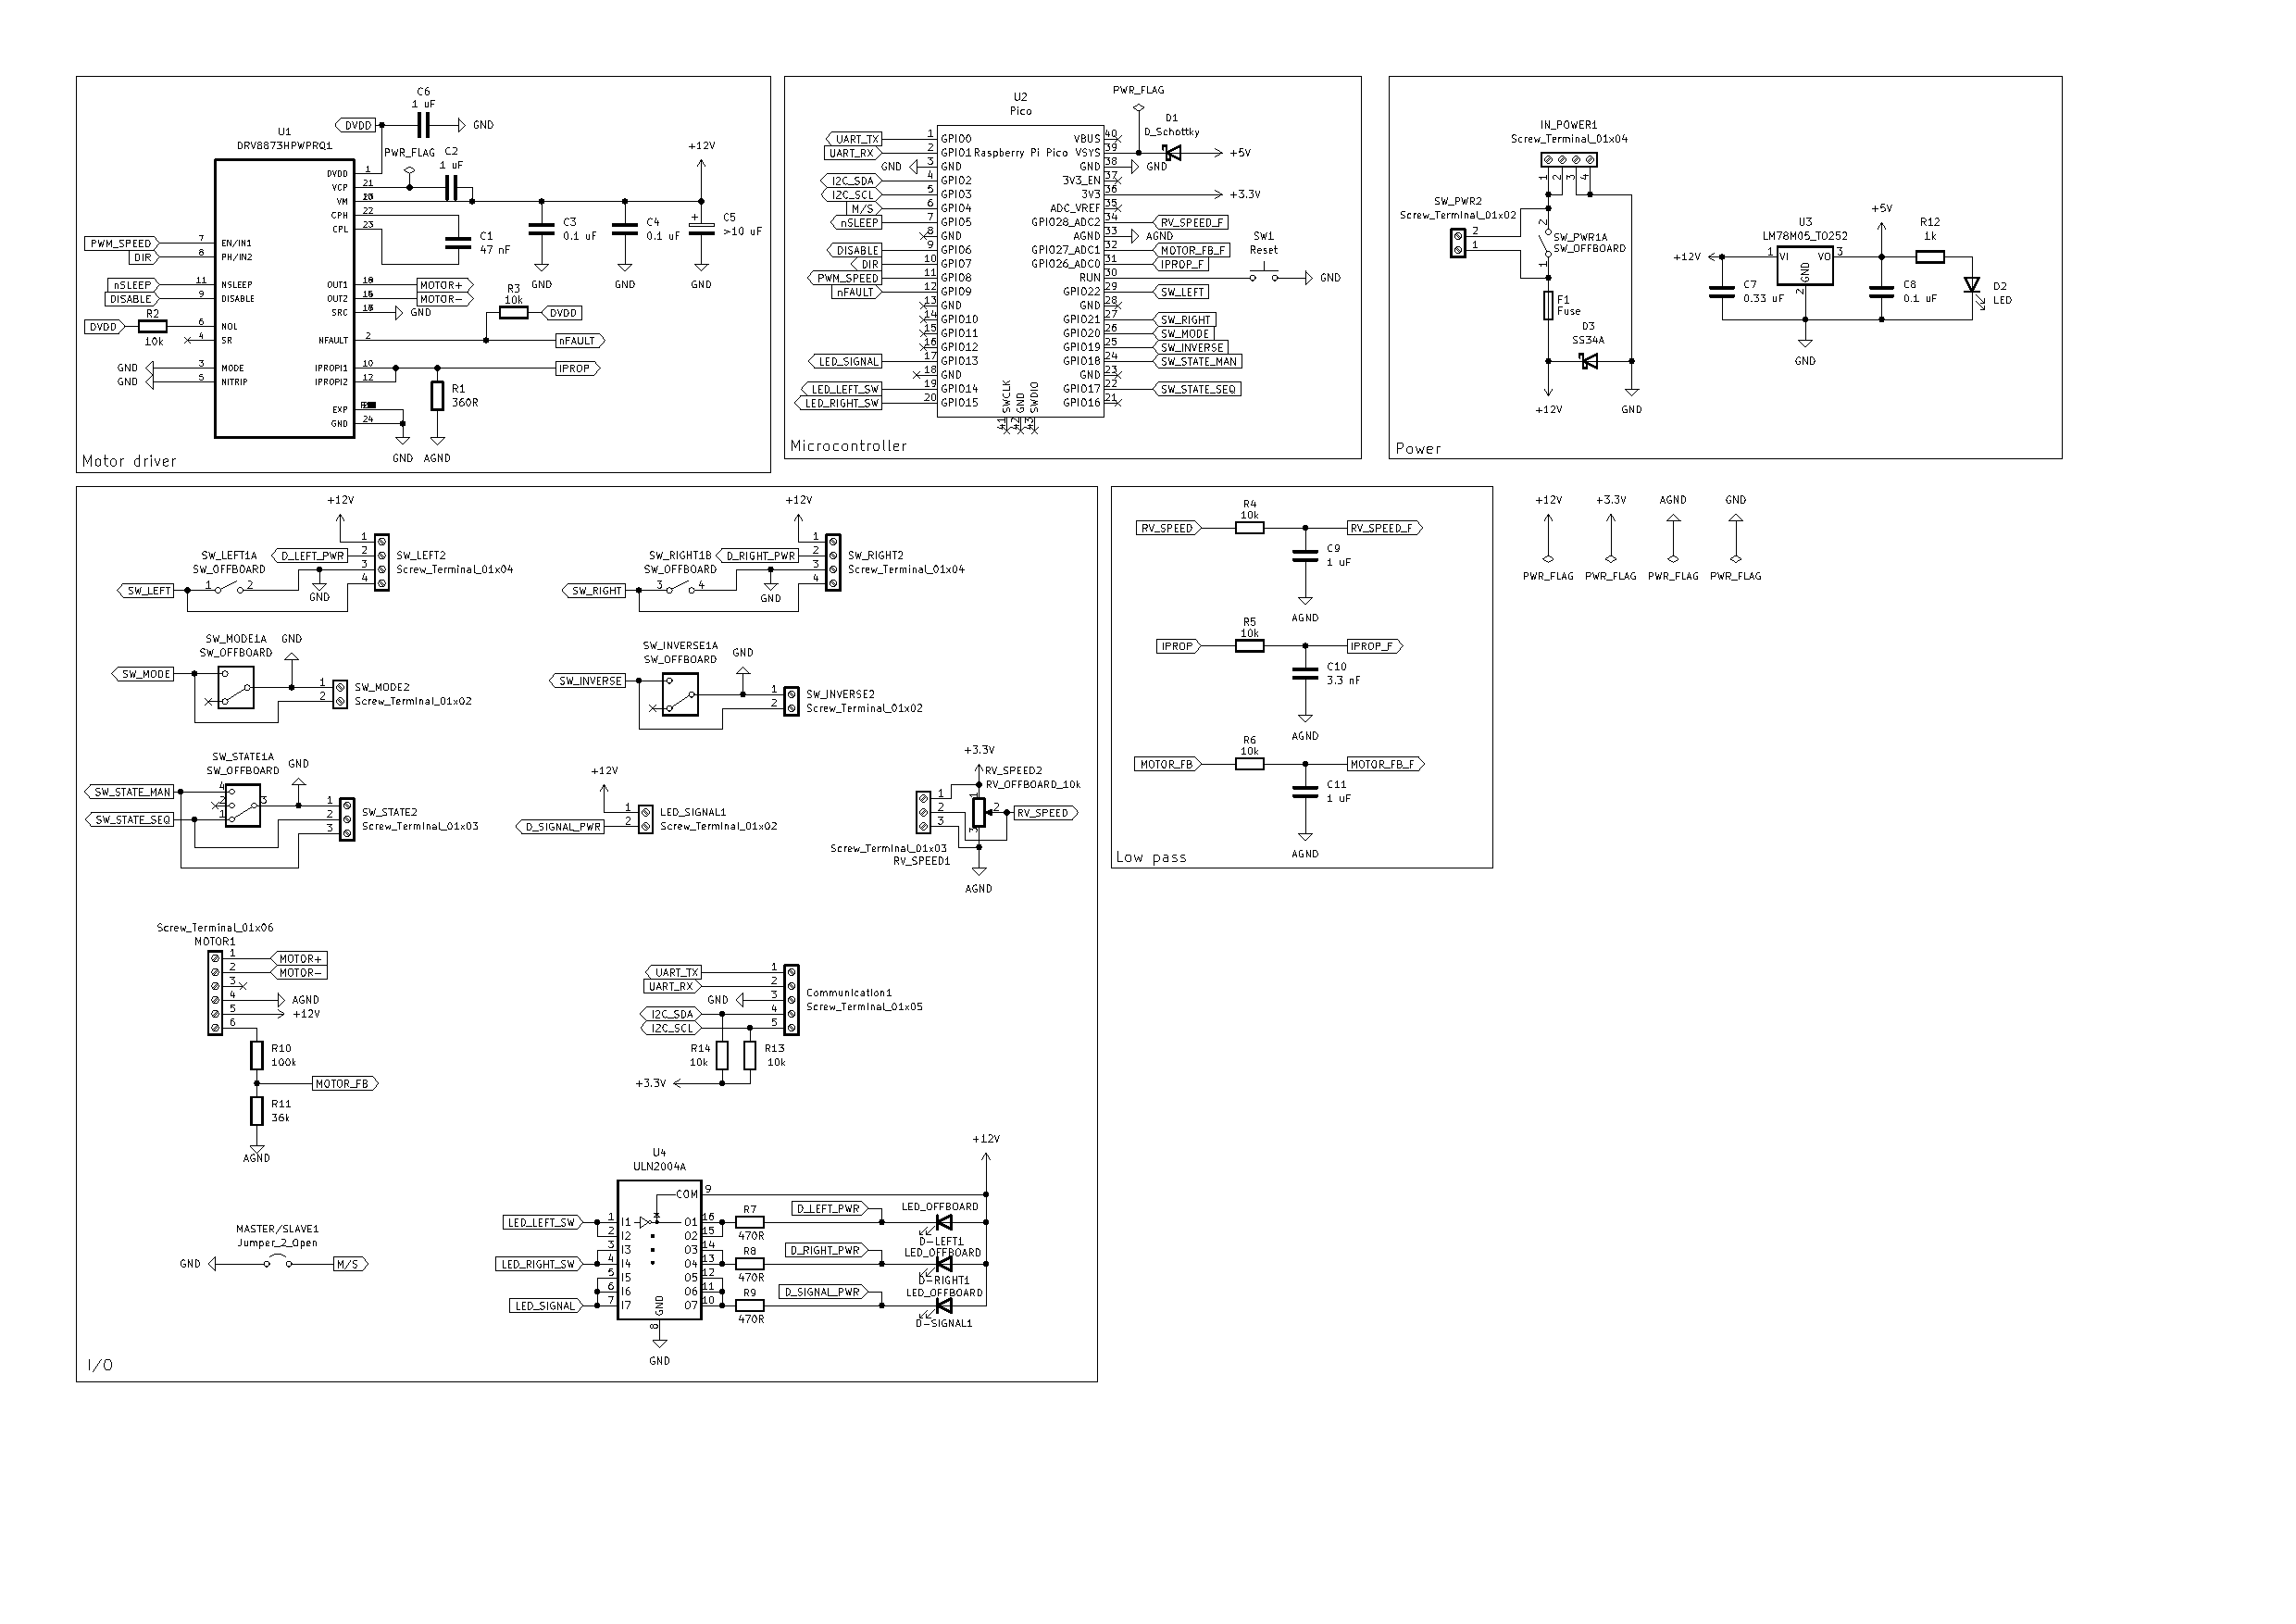
\includepdf[pages=-,landscape]{images/1.0.0_20250715.pdf}

\begin{figure}[h!]
    \centering
    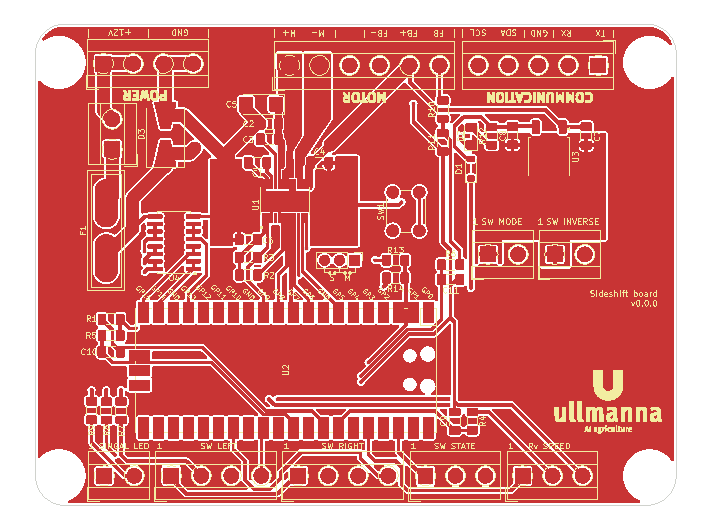
\includegraphics[width=0.92\textwidth]{images/siteshift-F_Cu.pdf}
\end{figure}

\begin{figure}[h!]
    \centering
    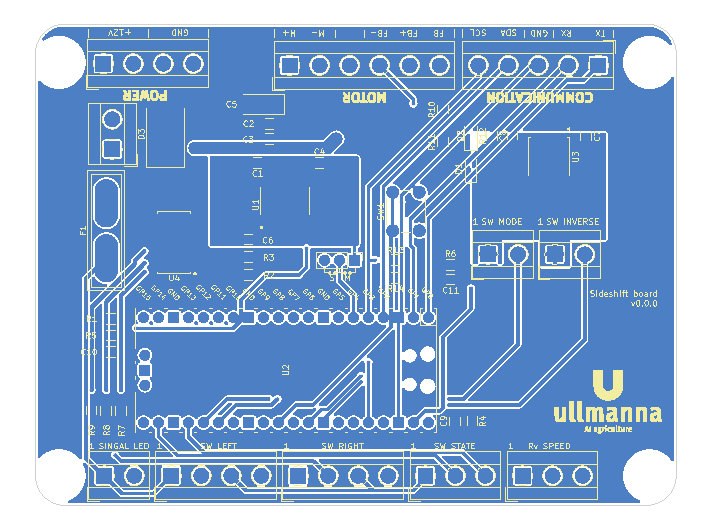
\includegraphics[width=0.92\textwidth]{images/siteshift-B_Cu.pdf}
\end{figure}





\end{document}
